\section{Design Patterns}
  \subsection{Architetturali}
    \subsubsection{Architettura a microservizi}
      \begin{itemize}
       \item \textbf{Scopo:} l'architettura a \gl{microservizi} è un approccio allo sviluppo di una singola applicazione come insieme di piccoli servizi, ciascuno dei quali viene eseguito da un proprio processo e comunica con un meccanismo snello, spesso una \gl{HTTP} \gl{API};
       \item \textbf{Vantaggi:}
	      \begin{itemize}
	       \item ogni \gl{microservizio} è relativamente piccolo, quindi più semplice da implementare e da capire per gli sviluppatori;
	       \item ogni microservizio è indipendente dagli altri; è quindi possibile distribuire nuove versioni più frequentemente e isolare i possibili errori.
	      \end{itemize}

       \item \textbf{Svantaggi:}
	\begin{itemize}
	 \item l'architettura risulta maggiormente complessa perchè risulta essere un \gl{sistema} distribuito;
	 \item la gestione di più microservizi potrebbe risultare in un carico di lavoro maggiore rispetto ad una sua versione monolitica.
	\end{itemize}
      \end{itemize}
      \begin{figure}[h]
      	\centering
      	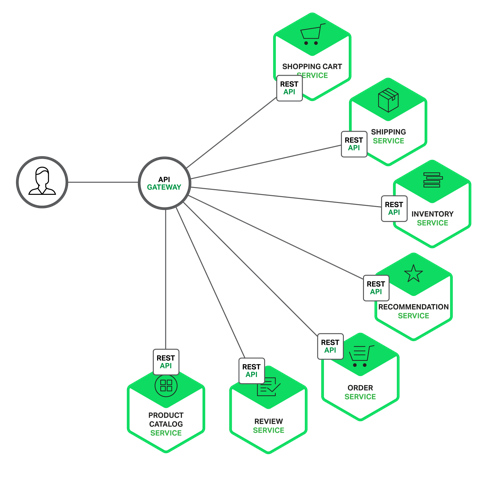
\includegraphics[width=\textwidth,height=\textheight,keepaspectratio,scale=0.1]{images/micros.png}
      	\caption{Architettura a microservizi}\label{fig:micr1}
      \end{figure}
      \newpage
    \subsubsection{Architettura event-driven}
      \begin{itemize}
       \item \textbf{Scopo:} anche se non è un vero e proprio pattern, l'architettura \gl{event-driven} è un particolare tipo di architettura asincrona per sistemi distribuiti basata sugli eventi;
	\item \textbf{Vantaggi:}
	  \begin{itemize}
	   \item per definizione, questo tipo di architettura è particolarmente adatto ad ambienti di tipo asincrono basati sugli eventi, come ad esempio l'interazione con degli utenti in tempo reale;
	   \item permette un alto disaccoppiamento tra le componenti.
	  \end{itemize}
	\item \textbf{Svantaggi:}
	  \begin{itemize}
	   \item i sistemi che utilizzano tale architettura sono spesso distribuiti: ciò comporta un maggiore livello di complessità.
	  \end{itemize}
	\end{itemize}
    \subsubsection{Flux}
    \begin{itemize}
    	\item \textbf{Scopo:} questo pattern permette di gestire il flusso dei dati in un'applicazione, in particolare esso dovrà essere unidirezionale. Come visibile dal diagramma \ref{fig:flux}, abbiamo il Dispatcher che riceve delle Action, le quali verranno spedite agli Store registrati al Dispatcher. Successivamente, i dati presente negli Store saranno visualizzati tramite la View. Infine, da quest'ultima potranno essere inviate nuove Action al Dispatcher, riprendendo il flusso appena descritto.
    	\item \textbf{Vantaggi:}
    	\begin{itemize}
    		\item è totalmente indipendente dal linguaggio di programmazione utilizzato;
    		\item facilita il riuso delle componenti \gl{DOM}.
    	\end{itemize}
    	\item \textbf{Svantaggi:}
    	\begin{itemize}
    		\item non ha una buona curva d'apprendimento;
    		\item scrivere componenti DOM secondo questo pattern è verboso.
    	\end{itemize}
    \end{itemize}
    Alla pagina \url{https://github.com/facebook/flux/tree/master/examples/flux-concepts} (visitato in data 2017-03-26) è disponibile la documentazione ufficiale di questo pattern.\\
    In figura \ref{fig:flux} si ha il diagramma del pattern Flux, mentre in figura \ref{fig:flux2} si ha il diagramma dell'effettivo utilizzo del pattern all'interno dell'architettura progettata.\\
È utilizzato per la realizzazione di ConversationApp, la quale rappresenta l'applicazione di conversazione tra un utente e l'assistente virtuale.
    \begin{figure}[h]
    	\centering
    	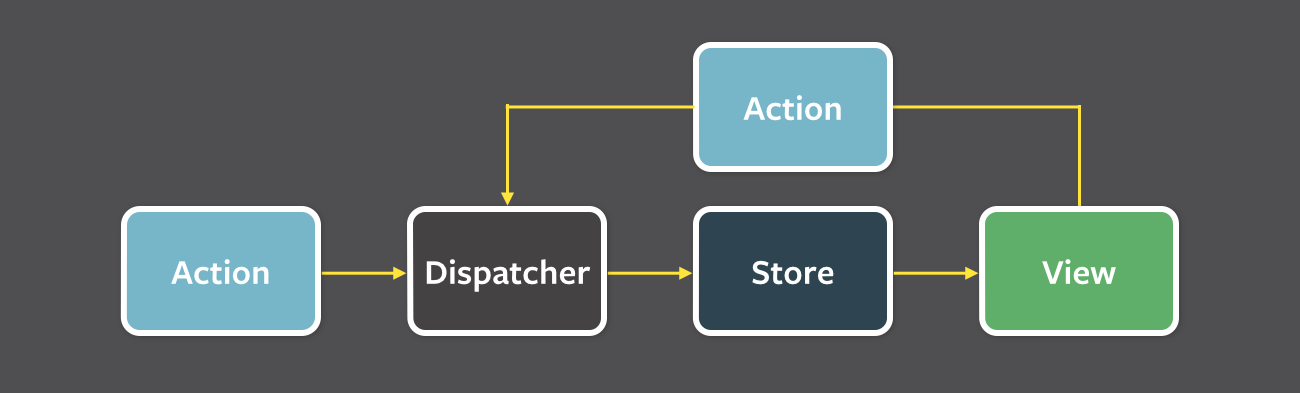
\includegraphics[width=\textwidth,height=\textheight,keepaspectratio]{images/fluxpattern.png}
    	\caption{Pattern flux}\label{fig:flux}
    \end{figure}
    \begin{figure}[h]
	\centering
	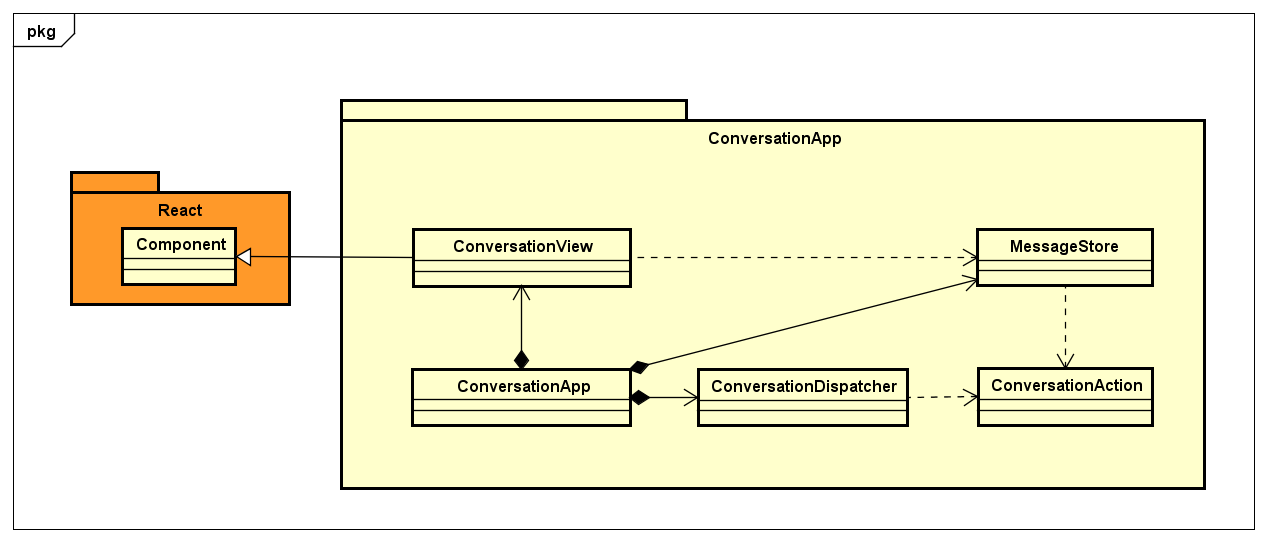
\includegraphics[width=\textwidth,height=\textheight,keepaspectratio,scale=0.1]{images/diagrams/client/Client/Flux.png}
	\caption{Flux utilizzato nell'architettura del \gl{progetto} \PROGETTO}\label{fig:flux2}
\end{figure}
    \newpage

    \newpage
   \subsubsection{Data Access Object}
      \begin{itemize}
       \item \textbf{Scopo:} il pattern \gl{Data Access Object} (DAO) consiste nell'utilizzo di un oggetto che fornisce un'interfaccia astratta per la gestione di una sorgente di dati, o più in generale per la gestione della persistenza.
	\item \textbf{Vantaggi:}
	  \begin{itemize}
	   \item separazione tra logica di business e dati;
	   \item modifiche alla struttura dei dati non comportano modifiche sul client che utilizza DAO.
	  \end{itemize}
	\item \textbf{Svantaggi:}
	  \begin{itemize}
	   \item un'interfaccia di questo tipo potrebbe nascondere i costi di accesso ad un database;
	   \item potrebbero essere necessarie molte più operazioni rispetto all'esecuzione diretta di una query su un database.
	  \end{itemize}
	\end{itemize}
In figura \ref{fig:dao1} si ha il diagramma del pattern DAO, mentre in figura \ref{fig:dao2} si ha il diagramma dell'effettivo utilizzo del pattern all'interno dell'architettura progettata.\\
È utilizzato per accedere a qualsiasi fonte di dati, ma sempre secondo lo schema in figura \ref{fig:dao2}, pertanto ne viene riportato solo il diagramma relativo all'interazione con la tabella \gl{DynamoDB} contenente le conversazioni registrate.
	\begin{figure}[h]
		\centering
		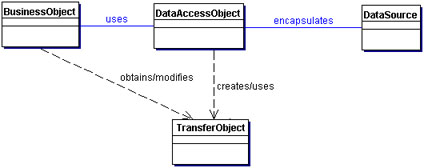
\includegraphics[width=\textwidth,height=\textheight,keepaspectratio,scale=0.1]{images/DAOpattern.jpg}
		\caption{pattern Data Access Object (DAO)}\label{fig:dao1}
	\end{figure}
\begin{figure}[h]
	\centering
	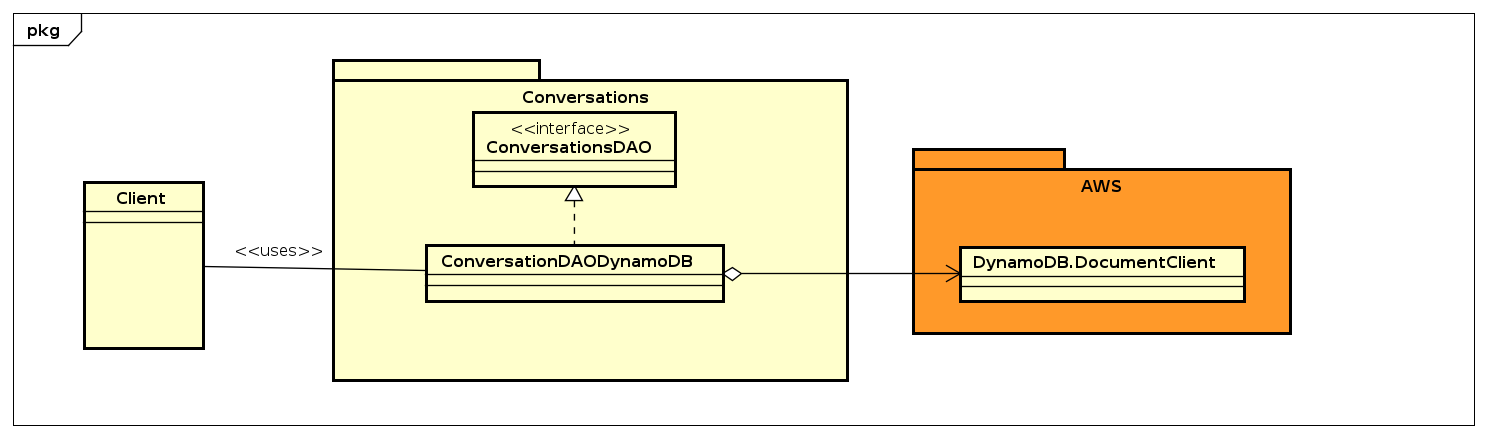
\includegraphics[width=\textwidth,height=\textheight,keepaspectratio,scale=0.1]{images/diagrams/back-end/DAO.png}
	\caption{DAO utilizzato nell'architettura del progetto \PROGETTO}\label{fig:dao2}
\end{figure}
		\newpage
    \subsubsection{Dependency Injection}
     \begin{itemize}
       \item \textbf{Scopo:} la \gl{dependency injection }consiste nella separazione del comportamento di una componente dalla risoluzione delle sue dipendenze.
	\item \textbf{Vantaggi:}
	  \begin{itemize}
	   \item la separazione del comportamento dalle dipendenze rende una componente molto più flessibile;
	   \item rende le singole componenti maggiormente indipendenti permettendo una più facile progettazione dei test di unità.
	  \end{itemize}
	\item \textbf{Svantaggi:}
	  \begin{itemize}
	   \item eventuali errori legati alla risoluzione delle dipendenze o alla loro implementazione vengono rilevati solamente a runtime;
	   \item rende più difficile il tracciamento del codice in quanto ne separa la costruzione dal comportamento.
	  \end{itemize}
	\end{itemize}

  \subsection{Strutturali}

    \subsubsection{Façade}
      \begin{itemize}
       \item \textbf{Scopo:}  indica un oggetto che permette, attraverso un'interfaccia più semplice, l'accesso a sottosistemi che espongono interfacce complesse e molto diverse tra loro, nonché a blocchi di codice complessi. \\
       Nel contesto della progettazione architetturale del progetto \PROGETTO, questo pattern non è stato usato nella sua forma pura (visibile in figura \ref{fig:facade}). Facendo però un utilizzo di un \gl{API Gateway}, il quale nasconde la complessità del back-end al client fornendone anche i meccanismi di utilizzo, si è fatto utilizzo dei concetti che questo pattern rispetta;
	\item \textbf{Vantaggi:}
	  \begin{itemize}
	   \item permette di nascondere la complessità di un'operazione: rispetto alla chiamata diretta di un sottoinsieme di classi è possibile chiamare solamente la classe definita come \gl{façade} semplificando l'operazione;
	   \item permette di diminuire le dipendenze tra sottosistemi;
	  \end{itemize}\newpage
	\item \textbf{Svantaggi:}
	  \begin{itemize}
	   \item i sottosistemi risultano essere collegati al façade: modifiche alla struttura dei sottosistemi comportano una serie di modifiche al façade stesso;
	  \end{itemize}
	\end{itemize}
	\begin{figure}[h]
		\centering
		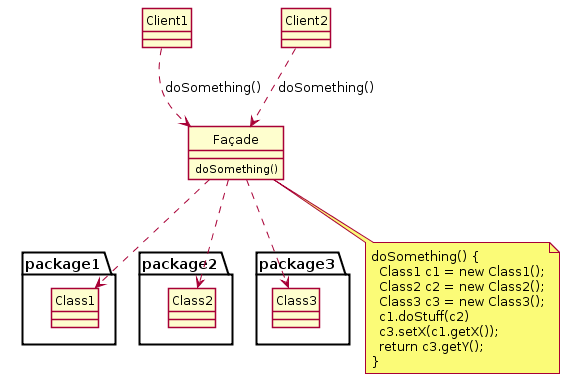
\includegraphics[width=\textwidth,height=\textheight,keepaspectratio,scale=0.1]{images/patternfacade.png}
		\caption{pattern Façade}\label{fig:facade}
	\end{figure}
    \subsubsection{Adapter}
      \begin{itemize}
       \item \textbf{Scopo:} questo pattern permette la comunicazione tra due interfacce completamente differenti tramite l'utilizzo di un Adapter.
	\item \textbf{Vantaggi:}
	  \begin{itemize}
	   \item permette la conversione di una classe esistente in un'altra completamente differente senza modificarne il codice;
	   \item maggiore flessibilità nella progettazione.
	  \end{itemize}
	\item \textbf{Svantaggi:}
	  \begin{itemize}
	   \item aumenta la dimensione del codice;
	   \item a volte per interconnettere due interfacce sono necessari più Adapter.
	  \end{itemize}
	\end{itemize}
	In figura \ref{fig:adapter1} si ha il diagramma del pattern Adapter, mentre in figura \ref{fig:adapter2} si ha il diagramma dell'effettivo utilizzo del pattern all'interno dell'architettura progettata.\\
È utilizzato per convertire l'interfaccia fornita da api.ai in una più adatta alle esigenze dell'applicazione, definita da \file{VAModule}. \\ La classe ApiAiVAAdapter, facendo da Adapter tra le API di api.ai (adaptee) e l'interfaccia \file{VAModule} (target), permette l'interoperabilità tra queste due interfacce.
	\begin{figure}[h]
		\centering
		
\includegraphics[width=\textwidth,height=\textheight,keepaspectratio,scale=0.1]{images/adapterpattern.png}
		\caption{Pattern Adapter}\label{fig:adapter1}
	\end{figure}
\begin{figure}[h]
		\centering
	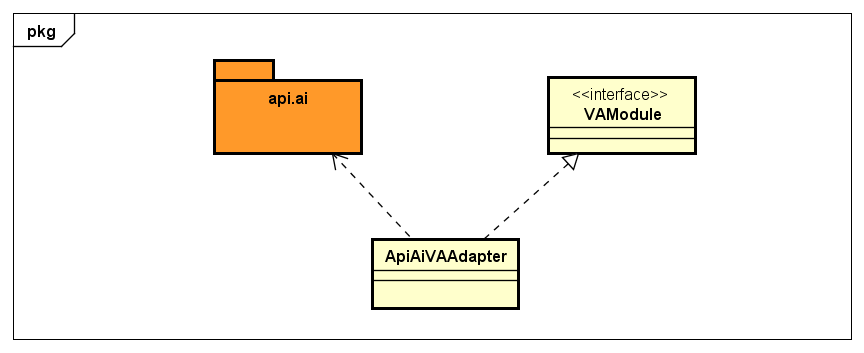
\includegraphics[width=\textwidth,height=\textheight,keepaspectratio,scale=0.1]{images/diagrams/back-end/Official_Backend_0304/Adapter.png}
	\caption{Adapter utilizzato nell'architettura del progetto \PROGETTO}\label{fig:adapter2}
\end{figure}
	\newpage
  \subsection{Creazionali}

	 \subsubsection{Module}
      \begin{itemize}
       \item \textbf{Scopo:} questo pattern ha lo scopo di introdurre il concetto di modularità nei linguaggi di programmazione che non lo possiedono.
	\item \textbf{Vantaggi:}
	  \begin{itemize}
	   \item come da definizione, questo pattern permette l'implementazione della modularità in ambienti privi di supporto ad essa.
	  \end{itemize}
	\item \textbf{Svantaggi:}
	  \begin{itemize}
	   \item la sua implementazione richiede un maggiore carico di lavoro.
	  \end{itemize}
	\end{itemize}
	  \newpage
  \subsection{Comportamentali}
    \subsubsection{Observer}
      \begin{itemize}
       \item \textbf{Scopo:} questo pattern, adottato nella variante offerta da ReactiveX, permette la definizione di una o più classi \gl{Observer} le quali "osservano" una classe Observable e ne gestiscono gli eventi.
	\item \textbf{Vantaggi:}
	  \begin{itemize}
	   \item permette la gestione di eventi tramite l'invio di dati ad altre classi in modo efficiente;
	   \item la definizione di classi Observer non causa modifiche alla classe Observable.
	  \end{itemize}
	\item \textbf{Svantaggi:}
	  \begin{itemize}
	   \item una cattiva implementazione comporta un aumento della complessità del codice;
	   \item l'interfaccia Observer deve essere implementata, e ciò comporta ereditarietà.
	  \end{itemize}
	\end{itemize}
	In figura \ref{fig:obs1} si ha il diagramma del pattern Observer, mentre in figura \ref{fig:obs2} si ha il diagramma dell'effettivo utilizzo del pattern all'interno dell'architettura progettata.\\
È utilizzato da diverse classi del sistema per osservare e gestire gli eventi generati dalle classi Subject, ma sempre secondo lo schema in figura \ref{fig:obs2}. Pertanto, come esempio, viene riportato solo il diagramma relativo alla relazione tra AgentObserver e AgentObservable.

	\begin{figure}[h]
		\centering
		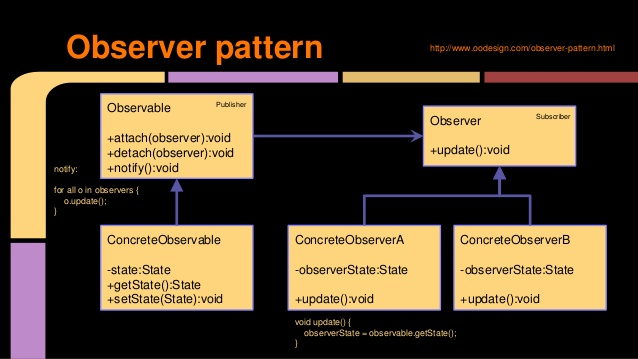
\includegraphics[width=\textwidth,height=\textheight,keepaspectratio,scale=0.1]{images/observerpattern.png}
		\caption{Pattern Observer}\label{fig:obs1}
	\end{figure}
	\begin{figure}[h]
		\centering
		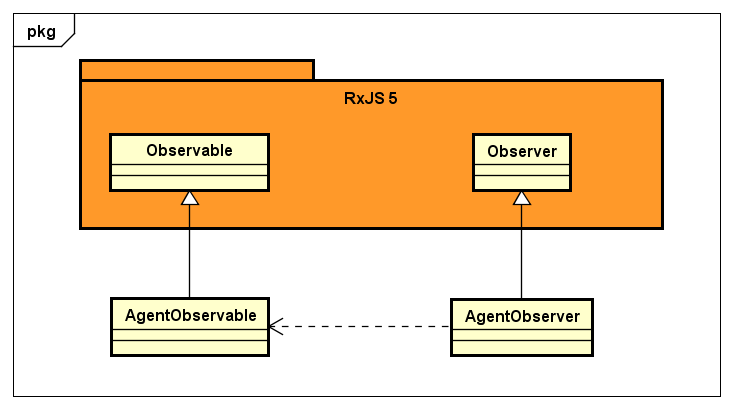
\includegraphics[width=\textwidth,height=\textheight,keepaspectratio,scale=0.1]{images/diagrams/back-end/Official_Backend_0304/Observer.png}
		\caption{Pattern Observer utilizzato nell'architettura del progetto \PROGETTO}\label{fig:obs2}
	\end{figure}
	\newpage
	\section{Tecnologie utilizzate}
	\subsection{Promise e Observable}


\gl{JavaScript} è un linguaggio single-threaded, quindi basato su un singolo thread in esecuzione. Questo significa dover aspettare sempre il termine di un'operazione prima di passare alla
successiva, quindi nel caso di operazioni di lunga durata, il flusso dell'elaborazione principale di un’applicazione JavaScript potrebbe "congelarsi". \\
Per aggirare questo problema, una delle soluzioni più diffuse è quella di passare una \gl{callback} alla funzione in questione e, anzichè aspettare il compimento dell'operazione, restituire
il controllo al chiamante. Al termine dell'operazione, la funzione di callback verrà invocata. \\


L'uso di callback, spesso annidate, rende il codice di difficile comprensione e di difficile manutenzione. Due possibili soluzioni sono l'uso delle Promise di bluebird e l'uso degli Observable
di RxJS.


\subsubsection{Promise e bluebird}

Una Promise è un oggetto che rappresenta il risultato in sospeso di un’operazione asincrona. Ciò permette ai metodi asincroni di restituire valori alla stessa maniera dei metodi sincroni:
invece del valore finale, il metodo asincrono restituisce una Promise, ovvero una promessa di ottenere un valore in un momento futuro. \\
I principali metodi di una Promise sono:

\begin{itemize}

\item \file{then}: ritorna una Promise, in questo modo è possibile concatenere successive chiamate a questo metodo. È composto da due parametri opzionali che corrispondono a
due funzioni: \file{onFulfill} viene richiamata se la Promise ha avuto successo, \file{onReject} se è stata rigettata.

\item \file{catch}: ritorna una Promise e si occupa di gestire eventuali errori generati nella catena dei \file{then}.

\end{itemize}
Si è deciso di utilizzare bluebird in quanto offre i seguenti vantaggi:

\begin{itemize}

\item cross-platform: ideale per progetti che prevedono esperienze multipiattaforma;

\item compatibile con le specifiche Promise/A+: bluebird può essere usato come rimpiazzo per Promise nativa offrendo un immediato miglioramento delle prestazioni;

\item debug facile: gli \gl{stack} trace in cui vengono riportati, quando possibile, gli errori non gestiti sono configurabili.

\end{itemize}

\subsubsection{Observable e RxJS v5}
ReactiveX è un insieme di API per estendere la programmazione asincrona facendo uso di Observable.\\
In base al linguaggio di programmazione che si vuole utilizzare, vengono fornite differenti librerie specifiche.
La scelta quindi ricade su RxJS, ReactiveX library per JavaScript.


Un Observable è una rappresentazione di un qualsiasi insieme di valori durante un qualsiasi periodo di tempo. Viene utilizzata per le implementazioni del pattern Observer.
RxJS v5 è ancora in beta ma sostituirà in breve la v4. Si è deciso di utilizzarla perchè è una libreria solida nella gestione degli Observable e sarà ulteriormente aggiornata
da Microsoft e altri sviluppatori di \gl{software} \gl{open source}.

I vantaggi sono:
\begin{itemize}
	\item semplifica la stesura del codice asincrono e la sua sintassi, migliorandone la leggibilità.
\end{itemize}
Gli svantaggi sono:
\begin{itemize}
	\item RxJS v5 è una libreria non ancora molto popolare, ma gode comunque di un buon supporto.
\end{itemize}

\subsection{AWS SDK per JavaScript in Node.js}

Data la scelta di appoggiarsi all'infrastruttura \gl{Amazon Web Services} (AWS) per lo sviluppo del sistema, il gruppo ha deciso di utilizzare l'AWS \gl{SDK} per JavaScript in \gl{Node.js} per
interfacciarsi ai singoli servizi offerti da AWS. Tale strumento permette di semplificare notevolmente l'utilizzo di tali servizi.

\subsubsection{Node.js}
La parte Back-End è stata sviluppata tramite la piattaforma event-driven Node.js, basata sul motore JavaScript V8. Esso permette di realizzare applicazioni Web utilizzando JavaScript, tipicamente utilizzato per applicazioni client-side, per la scrittura di applicazioni server-side. La caratteristica principale di Node.js risiede nel fatto che offre la possibilità di accedere alle risorse del sistema operativo in modalità event-driven non sfruttando il classico modello basato su processi o thread concorrenti utilizzato dai classici web server.\\
I vantaggi offerti sono:
\begin{itemize}
	\item approccio modulare, il quale permette un’organizzazione semplice del lavoro grazie alla combinazione di librerie con moduli importati.
\end{itemize}
Gli svantaggi sono:
\begin{itemize}
	\item approccio asincrono, il quale può dare delle difficoltà nell'apprendimento;
\end{itemize}

\subsubsection{Request promise}
Modulo di Node.js che offre il supporto alle richieste HTTP con l'approccio delle Promises. Il gruppo ha deciso di ricorrere all'utilizzo di tale modulo per rispettare la decisione di non utilizzare direttamente le funzioni di callback, ma ricorrere alle Promises.

\subsection{Amazon Web Services}
Di seguito sono elencati i servizi AWS che dovranno essere utilizzati.

\subsubsection{AWS Lambda}
\gl{AWS Lambda} è un servizio di \gl{cloud}-computing fornito da Amazon, il quale permette l'implementazione di una architettura \gl{serverless}. \\
Esso permette l'esecuzione di codice senza preoccuparsi della gestione di server o di tutte le risorse necessarie all'esecuzione del codice, in termini di tempo, spazio e computabilità. \\
AWS Lambda permette di eseguire codice su una piattaforma ad alta affidabilità, a patto che il codice sia scritto in un linguaggio supportato. Nel nostro caso, faremo utilizzo di Node.js 6.10, supportato da AWS Lambda. \\
Inoltre, questo servizio può essere utilizzato per eseguire del codice in risposta ad eventi. \\
La signature delle Lambda Function è la seguente:
\begin{verbatim}
function(event, context) {
    ...
}
\end{verbatim}
dove:
\begin{itemize}
	\item \file{event} è l'oggetto che contiene i dati della richiesta ricevuta dall'API Gateway. In particolare, contiene i seguenti campi:
	\begin{itemize}
		\item \file{body}: campo di tipo \file{String} contenente il corpo della richiesta;
		\item \file{pathParameters}: oggetto contenente i parametri passati all'API Gateway attraverso il path dell'\gl{URL};
		\item \file{urlQueryParameters}: oggetto contenente i parametri passati all'API Gateway attraverso query nell'URL.
	\end{itemize}
	\item \file{context} è l'oggetto contenente i dati relativi alla risposta e, in caso di Lambda Proxy Integration, contiene anche i seguenti metodi:
	\begin{itemize}
		\item \file{succeed}: metodo da utilizzare per mandare una risposta all'API Gateway in caso di successo. La risposta dev'essere un oggetto contenente i seguenti campi:
		\begin{itemize}
			\item \file{headers}: array associativo nel quale la chiave indica il nome di un header HTTP da mandare nella risposta, il quale valore associato è una stringa contenente il valore di tale header;
			\item \file{statusCode}: attributo intero contenente il codice HTTP che dovrà avere la risposta;
			\item \file{body}: stringa contenente il corpo della risposta da mandare.
		\end{itemize}
	\end{itemize}
\end{itemize}

\subsubsection{DynamoDB}
Amazon DynamoDB è un servizio che fornisce un database \gl{NoSQL}, il quale permette di immagazzinare documenti e grafici tra i suoi dati. E' veloce e flessibile, ideato per tutte le applicazioni che richiedono una latenza costante non superiore a una decina di millisecondi, e grazie alle sue caratteristiche si presta perfettamente come supporto per applicazioni Web.\\
È un servizio di database NoSQL cloud interamente gestito, è quindi sufficiente creare una tabella di database, impostare il throughput desiderato e lasciare che il servizio si occupi del resto. \\
I vantaggi offerti sono:
\begin{itemize}
	\item prestazioni rapidi e costanti, in media non oltre una decida di millisecondi;
	\item alta scalabilità, in quanto è possibile ridimensionare i requisiti di throughput,
	\item sicurezza, in quanto vengono forniti dei meccanismi per il controllo granulare degli accessi degli utenti;
	\item flessibilità, in quanto sono supportate sia le strutture di dati di tipo documento sia quelle di tipo chiave-valore;
\end{itemize}
Gli svantaggi sono:
\begin{itemize}
  \item rispetto ad altri database NoSQL, le funzioni offerte sono più limitate;
	\item non è un servizio gratuito, ma i costi sono legati a tariffe basate sul consumo effettivo, senza pagamenti anticipati né impegni di lungo termine.
\end{itemize}
\subsubsection{API Gateway}
Amazon API Gateway è un servizio completamente gestito che semplifica agli sviluppatori la creazione, la pubblicazione, la manutenzione, il monitoraggio e la protezione delle API su qualsiasi scala.\\
In questo modo, si può fornire una porta d'entrata attraverso la quale le applicazioni possono accedere a dati, logica di business o funzionalità dei servizi di back-end.\\
I vantaggi offerti sono:
\begin{itemize}
	\item alte prestazioni e scalabilità, offrendo una bassa latenza sulle richieste API e relative risposte;
	\item un pannello di controllo che consente di monitorare visivamente le chiamate al servizio;
	\item esecuzione simultanea di diverse versioni della stessa API, consentendo di iterare, testare e rilasciare nuove versioni in tempi brevi;
	\item strumenti per concedere le autorizzazioni di accesso alle API e controllare l'accesso alla gestione dei servizi;
	\item creazione di \gl{endpoint} \gl{REST}, permettendo di creare API avanzate basate sulle risorse, impiegando poi le dinamiche e flessibili funzionalità di trasformazione dei dati per generare le richieste nel linguaggio dei servizi a cui le richieste sono rivolte;
	\item esecuzione di API serverless, ista l'integrazione con AWS Lambda.
\end{itemize}
Gli svantaggi sono:
\begin{itemize}
	\item non è un servizio gratuito, ma ha dei costi calcolati in base alle chiamate effettuate alle API ed in base alla mole di dati in uscita trasferiti.
\end{itemize}

\subsubsection{SNS}
Amazon Simple Notification Service (Amazon SNS) è un servizio di notifiche push rapido, flessibile e completamente gestito che consente di inviare messaggi individuali o collettivi a un numero elevato di destinatari. \\
Con Amazon SNS è possibile inviare notifiche a dispositivi \gl{Apple}, Google, Fire OS e Windows. Inoltre, è possibile inviare notifiche push a delle Lambda Function  altri endpoint HTTP. \\
I vantaggi offerti sono:
\begin{itemize}
	\item alte prestazioni e affidabilità, infatti oltre ad avere una bassa latenza di risposta, tutti i messaggi pubblicati in Amazon SNS vengono memorizzati in modo ridondante su più server e data center;
	\item scalabilità, in quanto è consentita la pubblicazione di un altissimo numero di messaggi in qualsiasi momento;
	\item sicurezza, in quanto sono forniti meccanismi di controllo che permettono di proteggere argomenti e messaggi da accessi non autorizzati.
\end{itemize}
Gli svantaggi sono:
\begin{itemize}
	\item non è un servizio gratuito, ma ha costi legati al consumo effettivo.
\end{itemize}
\subsubsection{CloudWatch}
Amazon CloudWatch è un servizio di monitoraggio per le risorse cloud AWS e le applicazioni in esecuzione su AWS. Inoltre, tramite una semplice richiesta API, permette di inviare parametri personalizzati generati dalle proprie applicazioni per monitorarli tramite questo servizio.
\subsection{Serverless Framework}
Serverless Framework è un web \gl{framework} gratuito e open-source scritto tramite Node.js. Serverless è un framework per creare applicazioni esclusivamente su AWS Lambda. Un applicazione Serverless può essere composta da poche Lambda Functions per portare a termine semplici tasks o da molte Lambda Functions per creare ad esempio un intero back-end.\\
I vantaggi offerti sono:
\begin{itemize}
	\item semplifica lo sviluppo delle Lambda Function e dell'API Gateway di AWS;
  \item ha una community di supporto molto attiva.
\end{itemize}
Gli svantaggi sono:
\begin{itemize}
	\item è un framework molto recente, e di conseguenza non molto maturo.
\end{itemize}

\subsection{JWT}
JWT è uno standard basato su \gl{JSON} per creare token di accesso che possono sostenere richieste. I token sono firmati dalla chiave del server, quindi il client può verificare se un token è legittimo. I token sono pensati per essere compatti, senza contenere caratteri invalidi per gli URL e usabili principalmente nei contesti \gl{Single sign-on} (SSO).Le richieste JWT possono essere usate solitamente per passare l'identità di un utente autenticato tra un identity provider e un service provider. I token inoltre possono essere autenticati e criptati.\\
I vantaggi offerti sono:
\begin{itemize}
	\item alto grado di sicurezza nella trasmissione delle informazioni in formato JSON;
	\item la gestione dei token è notevolmente semplificata.
\end{itemize}
Gli svantaggi sono:
\begin{itemize}
	\item l'algoritmo crittografico per verifica i dati è molto complesso.
\end{itemize}
\subsection{Web Speech API}
Web Speech API fornisce fornisce due aree distinte di funzionalità, il riconoscimento vocale e la sintesi vocale (conosciuta anche come \gl{text to speech} o tts).
Il riconoscimento vocale è acceduto attraverso l'interfaccia SpeechRecognition, la quale fornisce la possibilità di riconoscere il contesto vocale da un input vocale e risponde appropriatamente.
La sintesi vocale è acceduta tramite l'interfaccia SpeechSynthesis, una componente text-to-speech che permette ai programmi di leggere testo.

\subsection{Speaker recognition}
Speaker Recognition API è un servizio Microsoft che, dopo aver costruito l'impronta vocale di un individuo, permette l'autenticazione per mezzo della voce. Al suo interno utilizza JSON per lo scambio dei dati e API Keys per l'autenticazione.
\\
I vantaggi offerti sono:
\begin{itemize}
	\item l'affidabilità del riconoscimento vocale è molto alta.
\end{itemize}
Gli svantaggi sono:
\begin{itemize}
	\item dopo le 10.000 chiamate al servizio al mese, il servizio non è più gratuito.
\end{itemize}
\subsection{STT IBM Watson}
Lo Speech to Text Watson è un servizio di IBM che, dato un file audio in input, restituisce il testo pronunciato in esso. Per trascrivere la voce umana accuratamente il servizio utilizza il \gl{machine learning} per combinare informazioni riguardo la grammatica e la struttura del linguaggio con la composizione del segnale audio. Il servizio fornisce trascrizioni sempre migliori in base a quanto dialogo viene ascoltato.
I vantaggi offerti sono:
\begin{itemize}
	\item l'affidabilità del riconoscimento vocale è molto alta.
\end{itemize}
Gli svantaggi sono:
\begin{itemize}
	\item dopo 1000 minuti di utilizzo  al mese, il servizio non è più gratuito.
\end{itemize}
\subsection{api.ai}
È una piattaforma di conversazione che permette interazioni sofisticate con il linguaggio naturale.\\
Le applicazioni sviluppate su questa piattaforma sono costuite da Agent, i quali si occupano di trasformare il linguaggio naturale in dati processabili. Tali Agent sono a loro volta costituiti da Intent, che hanno il compito di associare la richiesta dell'utente ad una determinata azione del software, ed Entity, che sono strumenti per estrarre dal linguaggio naturale i parametri attesi.\\
I vantaggi offerti sono:
\begin{itemize}
	\item lo sviluppo di un assistente avanzato è piuttosto semplice.
\end{itemize}
Gli svantaggi sono:
\begin{itemize}
	\item accetta solo input di tipo testuale.
\end{itemize}
\subsection{React}
React è una libreria cross-platform open-source per JavaScript, sviluppata da Facebook, che permette di creare interfacce utente. Esso supporta e realizza il pattern architetturale Flux (Visibile in figura \ref{fig:flux}). \\
La sua sintassi è chiamata JSX, la quale consiste nel combinare codice HTML con quello JavaScript, con lo scopo di velocizzare la scrittura del codice.\\
I vantaggi offerti sono:
\begin{itemize}
	\item è estremamente efficiente;
	\item vengono fornite delle estensioni per facilitare il debugging;
	\item facilita la scrittura di test per l'interfaccia utente.
\end{itemize}
Gli svantaggi sono:
\begin{itemize}
	\item l'integrazione con altri pattern tradizionali, ad esempio Model-View-Controller (MVC), risulta complessa;
	\item non ha una buona curva d'apprendimento.
\end{itemize}
\subsection{HTML5}
\gl{HTML5} è un linguaggio di \gl{markup} per la strutturazione di pagine web, pubblicato dal W3C nell’ottobre del 2014 con lo scopo di migliorare l’HTML4, permettendo supporto a nuovi file multimediali, mantenendo la leggibilità da parte di uomini e computer.
I vantaggi offerti sono:
\begin{itemize}
	\item è uno stantard W3C.
\end{itemize}
Gli svantaggi sono:
\begin{itemize}
	\item non è supportato da tutti i vecchi \gl{browser}.
\end{itemize}
\subsection{CSS3}
Pubblicata nel novembre 2014 dal W3C, \gl{CSS3} è una versione di CSS che va a correggere alcuni bug di interpretazione di Internet Explorer, migliorare la gestione degli sfondi e una soluzione per realizzare i bordi arrotondati.\\
CSS3 è suddiviso in moduli, al contrario delle versioni monolitiche precedenti, contenenti le vecchie specifiche CSS e nuove caratteristiche. Ciascun modulo tratta un tema diverso inerente i fogli di stile e, di conseguenza, ciascun tema è sviluppato in tempistiche differenti.
\subsection{Sass}
Sass è un linguaggio di scripting interpretato in CSS. Viene utilizzato per semplificare la lettura e la scrittura di fogli di stile CSS. Fornisce le seguenti funzionalità:

\begin{itemize}

\item definizione di variabili, per il riutilizzo di informazioni;

\item annidamento dei selettori;

\item ereditarietà dei selettori;

\item possibilità di utilizzo di operatori matematici;

\item possibilità di includere file Sass all'interno di altri file Sass che il browser interpreterà come un singolo file CSS, aumentandone la modularità;

\end{itemize}

A causa di queste funzionalità, il gruppo ha deciso di utilizzare tale tecnologia per i fogli di stile, invece di utilizzare direttamente il linguaggio CSS3.
